%==================================================================================================
\chapter{Movimentação da malha via suavização de Laplace} \label{MovMalha}
%==================================================================================================

Para a solução de problemas de IFE por meio da descrição ALE, se faz necessária a movimentação do domínio computacional do fluido de forma a acomodar a movimentação de estrutura. Tal tarefa deve ser realizada mantendo-se a qualidade da malha utilizada para o cálculo dos passos de tempo posteriores, evitando, assim, distorções excessivas nos elementos. Como mencionado por \citeonline{kanchi20073d}, essa etapa deve produzir uma malha de boa qualidade ao longo do tempo, ao mesmo tempo que não deve ser custoso computacionalmente. Assim, uma possibilidade para se realizar a movimentação da malha parte da suavização de Laplace, o qual foi estudado tanto em casos bidimensionais \cite{masud2007adaptive}, quanto tridimensionais \cite{kanchi20073d}.

Nesse esquema, considere o domínio limitado aberto do fluido $\Omega_F$, com uma fronteira suave por partes $\Gamma$. Logo, $\Gamma$ pode ser decomposta em partes de fronteira fixa $\Gamma_f$ e partes de fronteira móvel $\Gamma_m$, tais que:

\begin{subequations}
    \begin{equation}
        \Gamma=\Gamma_m\cup\Gamma_f\text{ e}
    \end{equation}
    \begin{equation}
        \varnothing=\Gamma_m\cap\Gamma_f\text{.}
    \end{equation}
\end{subequations}

Dessa forma, define-se as condições de contorno do problema como:

\begin{equation}
    \left\{
    \begin{array}{ll}
        \BB{z}=\BB{z}_m & \text{ em }\Gamma_m\text{ e} \\
        \BB{z}=\BB{0}   & \text{ em }\Gamma_f\text{,}
    \end{array}
    \right.
\end{equation}

\noindent em que $\BB{z}$ é o campo de deslocamentos da malha e $\BB{z}_m$ é o deslocamento prescrito em $\Gamma_f$.

Em seu trabalho, \citeonline{masud2007adaptive} aprontam que a simples utilização de uma equação do tipo $\Lapl\BB{z}=\BB{0}$ em $\Omega_F$ apresenta uma boa movimentação da malha em situação onde os elementos possuem tamanhos semelhantes entre si, assim como $\BB{z}_m$ não apresenta uma ordem de grandeza muito superior ao tamanho dos elementos na interface $\Gamma_m$. No entanto, como destacado pelos autores, a malha do fluido possui um refinamento maior em áreas de interesse da análise, o que coincide, em muitos casos, com a região próxima à $\Gamma_m$. Assim, se propõe uma modificação na formulação para que os elementos menores não sofram grandes distorções e inversões, ao passo que os elementos maiores absorverão tais distorções.

Assim, propõe-se um esquema de movimentação dado pelo problema de valor de contorno:

\begin{equation}
    \left\{
    \begin{array}{ll}
        \Nx\cdot([1+\eta]\Nx)\BB{z}=0 & \text{ em }\Omega_F\text{,}  \\
        \BB{z}=\BB{z}_m               & \text{ em }\Gamma_m\text{ e} \\
        \BB{z}=\BB{0}                 & \text{ em }\Gamma_f\text{,}
    \end{array}
    \right.\label{eq:LaplMov}
\end{equation}

\noindent em que:

\begin{equation}
    \eta^e=\frac{V_\mathrm{máx}-V_\mathrm{mín}}{V^e}
    \label{eq:movStiff}
\end{equation}

\noindent é um termo adicionado ao problema de maneira a aumentar a rigidez dos elementos menores, enquanto possibilita a movimentação dos elementos maiores, $V_\mathrm{máx}$, $V_\mathrm{mín}$ e $V^e$ são os volumes atuais do maior elemento, do menor elemento e do elemento $e$ calculado.

Para a solução do problema \eqref{eq:LaplMov}, parte-se para o método dos resíduos ponderados, em que $\BB{\upsilon}$ é a função teste:

\begin{equation}
    \SintDom{[1+\eta^e]\BB{\upsilon}\cdot\Laplx\BB{z}}=0\text{.}
\end{equation}

Integrando por partes e aplicando o teorema da divergência tem-se que:

\begin{equation}
    \SintFront{[1+\eta^e]\BB{\upsilon}\cdot(\Nx\BB{z}\cdot\BB{n})}-\SintDom{[1+\eta]\Nx\BB{\upsilon}:\Nx\BB{z}}=0\text{.}
\end{equation}

Por se tratar de um problema de fronteira de Dirichlet, a primeira parcela é nula, o que leva ao seguinte problema:

\begin{equation}
    \SintDom{[1+\eta^e]\Nx\BB{\upsilon}:\Nx\BB{z}}=0\text{.}
\end{equation}

Fazendo a aproximação da função teste por funções de forma, tem-se:

\begin{equation}
    \sum_{e=1}^{n_{el}}{\BB{\Upsilon}_a\cdot\intDome{[1+\eta^e](\Nx N_a\cdot\Nx)\BB{z}}}\text{,}
\end{equation}

\noindent sendo $\BB{\Upsilon}_a$ e $N_a$ o valor nodal da função teste e a função de forma sobre o nó $a$.

Devido à arbitrariedade da função teste, tem-se, portanto, a definição do vetor resíduo do problema de Laplace:

\begin{equation}
    \res_L^a=\intDome{[1+\eta^e](\Nx N_a\cdot\Nx)\BB{z}}=0\text{.}
    \label{eq:resLapl}
\end{equation}

Para se determinar o vetor $\BB{Z}$, referente aos deslocamentos nodais da malha, parte-se para o método de Newton-Raphson. Assim, toma-se como variáveis a serem corrigidas as acelerações nodais, que, a partir de uma aproximação por $\alpha$-generalizado tem-se a seguinte matriz do problema:

\begin{equation}
    \BB{B}^{ab}=\der{\res_L^a}{\ddBB{Y}^b}=\alpha_f\beta\Delta t^2\intDome{[1+\eta^e]\Nx N_a\cdot\Nx N_b}\BB{I}\text{.}
    \label{eq:movMatriz}
\end{equation}

Portanto o problema de movimentação da malha no contexto do MEF pode ser dado por:

\begin{equation}
    \BB{B}\Delta\ddBB{Y}=-\res_L\text{,}
    \label{eq:sistLapl}
\end{equation}

\noindent sujeito às seguintes condições de contorno:

\begin{equation}
    \left\{
    \begin{array}{ll}
        \ddBB{y}=\ddBB{y}_m & \text{ em }\Gamma_m \\
        \ddBB{y}=\BB{0}     & \text{ em }\Gamma_f
    \end{array}
    \right.
\end{equation}

Assim, o procedimento utilizado para a movimentação da malha é apresentado no algoritmo \ref{alg:movMalha}.

\begin{algorithm}[h!]
    \caption{Algoritmo utilizado para realizar a movimentação da malha.}
    \label{alg:movMalha}
    \ForEach{\textnormal{passo de tempo}}{
    % Previsão dos valores nodais:\newline
    % $
    %     \begin{bmatrix}
    %         \BB{y}^{n+1} \\\dBB{y}^{n+1}\\\ddBB{y}^{n+1}
    %     \end{bmatrix}^0\gets
    %     \begin{bmatrix}
    %         \BB{y}^n                                                                                    \\
    %         \bigpar{1-\frac{\gamma}{\beta}}\dBB{y}^n+\Delta t\bigpar{1-\frac{\gamma}{2\beta}}\ddBB{y}^n \\
    %         -\frac{\dBB{y}^n}{\beta\Delta t}+\bigpar{1-\frac{1}{2\beta}}\ddBB{y}^n
    %     \end{bmatrix}
    % $\\
    Atualização dos valores da fronteira\;
    \ForEach{\textnormal{iteração de Newton-Raphson}}{
    \ForEach{\textnormal{elemento}}{
        Interpolação das variáveis: $\BB{z}^{n+\alpha_f}\gets\alpha_f\BB{y}^{n+1}+(1-\alpha_f)\BB{y}^n-\BB{x}$\\
        Cálculo da matriz tangente \eqref{eq:movMatriz} e do vetor resíduo \eqref{eq:resLapl}\;
    }
    Montagem do sistema global e aplicação das condições de contorno\;
    Determinar as correções nodais pela solução do sistema \eqref{eq:sistLapl}\;
    Correção das acelerações: $(\ddBB{y}^{n+1})^{k+1}\gets(\ddBB{y}^{n+1})^k+\Delta(\ddBB{y}^{n+1})^k$\;
    Correção das posições e velocidades:\newline
    $
        \begin{bmatrix}
            \BB{y}^{n+1} \\\dBB{y}^{n+1}
        \end{bmatrix}^{k+1}\gets
        \begin{bmatrix}
            \BB{y}^n+\dBB{y}^n\Delta t+\Delta t^2\bigpar{\bigpar{\frac{1}{2}-\beta}\ddBB{y}^n+\beta\ddBB{y}^{n+1}} \\
            \dBB{y}^n+\Delta t\bigpar{(1-\gamma)\ddBB{y}^n+\gamma\ddBB{y}^{n+1}}
        \end{bmatrix}^{k+1}
    $\\
    Cálculo da medida de convergência $\epsilon$\;
    \lIf{$\epsilon<\mathrm{tol}$}{Sair do \textit{loop}}
    }

    Atualização dos valores passados\;
    }
\end{algorithm}

Uma outra possibilidade de movimentação pode ser obtida ao considerar o campo de acelerações da malha ao invés do campo de deslocamentos. Nesse caso, a equação que descreve a movimentação da malha é dada por:

\begin{equation}
    \left\{
    \begin{array}{ll}
        \Nx\cdot([1+\eta]\Nx\ddBB{y})=\BB{0} & \text{ em }\Omega_F\text{,}  \\
        \ddBB{y}=\ddBB{y}_m                  & \text{ em }\Gamma_m\text{ e} \\
        \ddBB{y}=\BB{0}                      & \text{ em }\Gamma_f\text{,}
    \end{array}
    \right.
    \label{eq:LaplMovAcc}
\end{equation}

\noindent em que $\ddBB{y}$ é o campo de acelerações da malha e $\ddBB{y}_m$ é o campo de acelerações prescrito em $\Gamma_f$.

Seguindo o mesmo procedimento descrito anteriormente, se obtém a seguinte expressão para o vetor resíduo:

\begin{equation}
    \res_L^a=\intDome{[1+\eta^e](\Nx N_a\cdot\Nx)\ddBB{y}}=0
    \label{eq:resLaplAcc}
\end{equation}

\noindent e a matriz tangente do problema:

\begin{equation}
    \BB{B}^{ab}=\der{\res_L^a}{\ddBB{Y}^b}=\alpha_m\intDome{[1+\eta^e]\Nx N_a\cdot\Nx N_b}\BB{I}
    \label{eq:movMatrizAcc}
\end{equation}

Portanto, se torna necessário apenas resolver o sistema \ref{eq:sistLapl} com essas novas expressões e aproximando o campo de deslocamentos via $\alpha$-generalizado.

%==================================================================================================
\section{Exemplos de verificação}
%==================================================================================================

Na sequência, são apresentados exemplos de aplicação do método de movimentação da malha por meio da suavização de Laplace. Para tanto, são estudados os problemas de cilindro com deslocamento prescrito, proposto por \citeonline{wan2007fictitious}, e o aerofólio com movimento de arfagem prescrito, proposto por \citeonline{mittal1992finite}.

%==================================================================================================
\subsection{Cilindro com deslocamento prescrito}
%==================================================================================================

O primeiro problema estudado é o cilindro com deslocamento prescrito, proposto por \citeonline{wan2007fictitious}. Nesse problema, um cilindro de raio $R=0,1\,\mathrm{m}$ encontra-se confinado em um canal definido por $\Omega=[-L/2, L/2]\times[0,H]$, com $L=2,2$ e $H=0,41$, sendo o centro do cilindro posicionado em $(0,\ 0,2)$. O movimento do cilindro ao longo do tempo é determinado por $y_1(t)=x_1+A\sin{(2\pi f t)}$, em que $A=0,25$ e $f=0,25$. As condições de contorno do problema são de paredes aderentes nas faces esquerda e direita do domínio, enquanto as faces superior e inferior são de paredes lisas. A Figura \ref{fig:moving-cylinder} apresenta o esquema do problema estudado.

\begin{figure}[h!]
    \centering
    \caption{Cilindro com deslocamento prescrito - Esquema do problema.}
    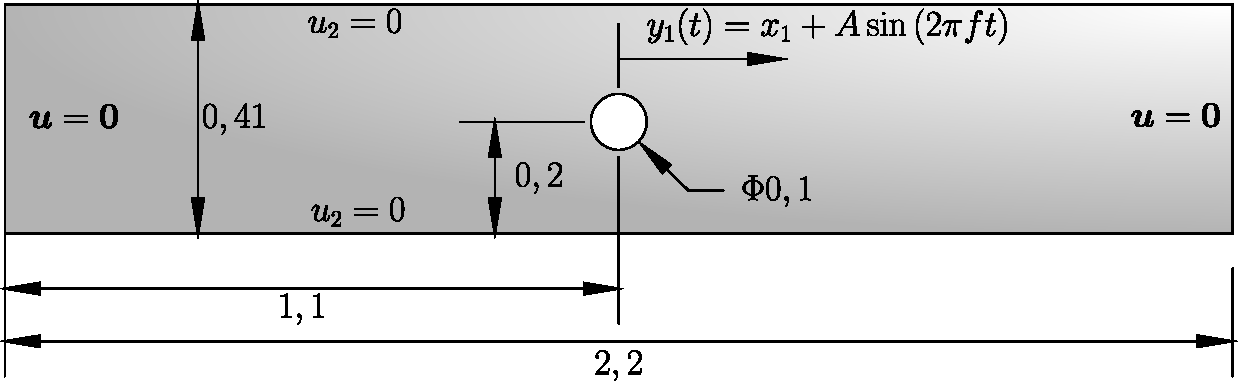
\includegraphics[width=.7\linewidth]{Figuras/moving-cylinder/moving-cilinder.pdf}
    \\Fonte: Autoria Própria (\the\year).
    \label{fig:moving-cylinder}
\end{figure}

O fluido possui viscosidade cinemática $\nu=1\times10^{-3}$, densidade $\rho=1,0$ e parte do repouso. O problema discretizado consiste na utilização de uma malha contendo 768 elementos triangulares de aproximação quadrática, totalizando 1664 nós e 4992 graus de liberdade. A simulação foi estabilizada por meio de SUPG/PSPG com esquema de integração temporal dado por $\rho_\infty=0,0$. O intervalo de tempo estudado é de $t\in[0,24]$ com passos de tempo $\Delta t=0,005$. A Figura \ref{fig:moving-cylinder-mesh} apresenta a configuração inicial da malha utilizada para a solução do problema.

\begin{figure}[h!]
    \centering
    \caption{Cilindro com deslocamento prescrito - Configuração inicial da malha.}
    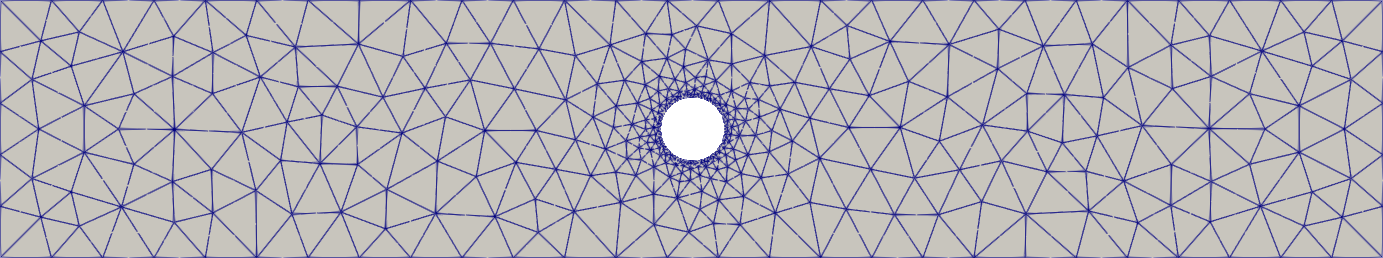
\includegraphics[width=\linewidth]{Figuras/moving-cylinder/mesh1.png}
    \\Fonte: Autoria Própria (\the\year).
    \label{fig:moving-cylinder-mesh}
\end{figure}

Assim, a malha é deformada no início de cada passo de tempo de forma a acomodar o movimento do cilindro. Assim, calcula-se o coeficiente de arrasto ao longo do tempo e compara-se com os resultados obtidos por \citeonline{wan2007fictitious}. A Figura \ref{fig:moving-cylinder-results} apresenta a comparação entre os resultados obtidos.

\begin{figure}[h!]
    \centering
    \caption{Cilindro com deslocamento prescrito - Coeficiente de arrasto ao longo do tempo.}
    \includegraphics[width=\linewidth]{Figuras/moving-cylinder/Cd.pdf}
    \\Fonte: Autoria Própria (\the\year).
    \label{fig:moving-cylinder-results}
\end{figure}

Verifica-se que os resultados obtidos possuem boa concordância com a referência, sendo observada apenas uma pequena diferença de fase entre os resultados, o que pode ser atribuído à diferença na condição inicial do problema.

As Figuras \ref{fig:moving-t-18-9} e \ref{fig:moving-t-21} apresentam as configurações da malha nos instantes $t=18,9$ e $t=21,0$, assim como os campos de velocidades obtidos nesses instantes.

\begin{figure}[h!]
    \centering
    \caption{Cilindro com deslocamento prescrito - Configuração da malha e campo de velocidades no instante $t=18,9$.}
    \begin{subfigure}{\linewidth}
        \centering
        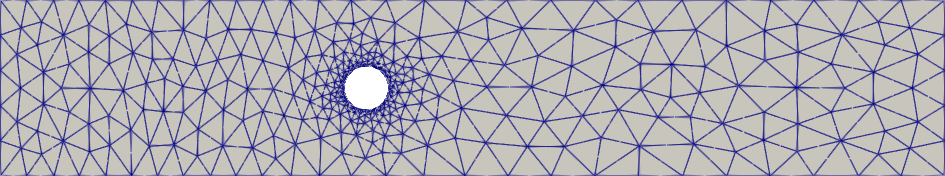
\includegraphics[width=\linewidth]{Figuras/moving-cylinder/m18-9.png}
        \caption{Configuração da malha.}
    \end{subfigure}
    \begin{subfigure}{\linewidth}
        \centering
        
\includegraphics[width=\linewidth]{Figuras/moving-cylinder/u18-9.png}
        \caption{Campo de velocidades.}
    \end{subfigure}
    \\Fonte: Autoria Própria (\the\year).
    \label{fig:moving-t-18-9}
\end{figure}

\begin{figure}[h!]
    \centering
    \caption{Cilindro com deslocamento prescrito - Configuração da malha e campo de velocidades no instante $t=21,0$.}
    \begin{subfigure}{\linewidth}
        \centering
        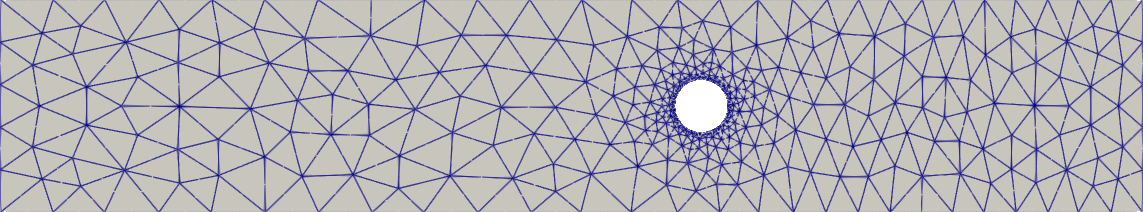
\includegraphics[width=\linewidth]{Figuras/moving-cylinder/m21.png}
        \caption{Configuração da malha.}
    \end{subfigure}
    \begin{subfigure}{\linewidth}
        \centering
        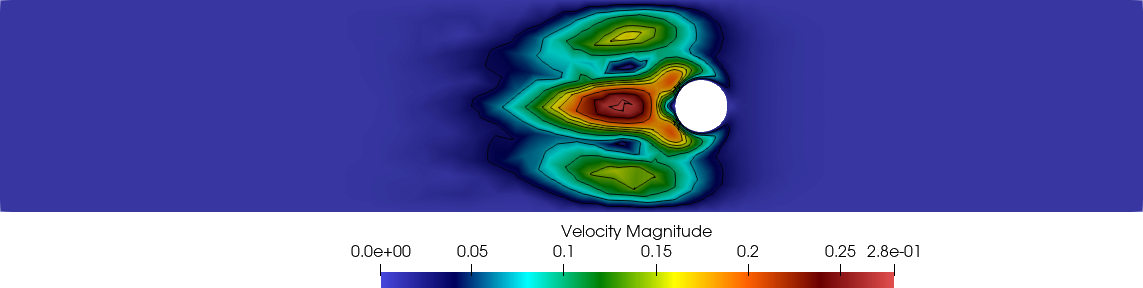
\includegraphics[width=\linewidth]{Figuras/moving-cylinder/u21.png}
        \caption{Campo de velocidades.}
    \end{subfigure}
    \\Fonte: Autoria Própria (\the\year).
    \label{fig:moving-t-21}
\end{figure}

Observa-se, portanto, que o esquema de movimentação da malha foi capaz de acomodar adequadamente o movimento do cilindro, assim como apresentou resultados muito próximos aos valores de referência, apontando a boa utilização do esquema de movimentação.

%==================================================================================================
\subsection{Aerofólio com movimento de arfagem}
%==================================================================================================

O exemplo seguinte se trata de um aerofólio NACA0012 com movimento de arfagem, proposto por \citeonline{mittal1992finite}, o qual aplica esse movimento como uma rotação prescrita do aerofólio em torno de um eixo. O domínio do problema é definido por $\Omega=[-9C, 21C]\times[-10C, 10C]$, com o centro geométrico do aerofólio posicionado em $(0,0)$. Inicialmente o aerofólio possui um ângulo de ataque ($\theta$) de $10,0^\circ$ e cujo valor varia ao longo do tempo por meio de:

\begin{equation}
    \theta(t)=\frac{\theta_\mathrm{máx}+\theta_\mathrm{mín}}{2}-\frac{\theta_\mathrm{máx}-\theta_\mathrm{mín}}{2}\cos{(\omega_f t)}\text{,}
\end{equation}

\noindent em que $\theta_\mathrm{máx}=30,0^\circ$ e $\theta_\mathrm{mín}=10,0^\circ$ são os valores máximo e mínimo do ângulo de ataque e $\omega_f=2\pi f_f$, sendo $f_f=1,0$ a frequência de oscilação. O giro do aerofólio se dá em torno de seu centro geométrico.

As condições de contorno do problema são de entrada na face esquerda ($\BB{u}=\{u_\infty,0\}\trans$), saída à direita e condição de simetria nas faces superior e inferior. A Figura \ref{fig:rotating-airfoil} apresenta o esquema do problema estudado.

\begin{figure}[h!]
    \centering
    \caption{Aerofólio com movimento de arfagem - Esquema do problema.}
    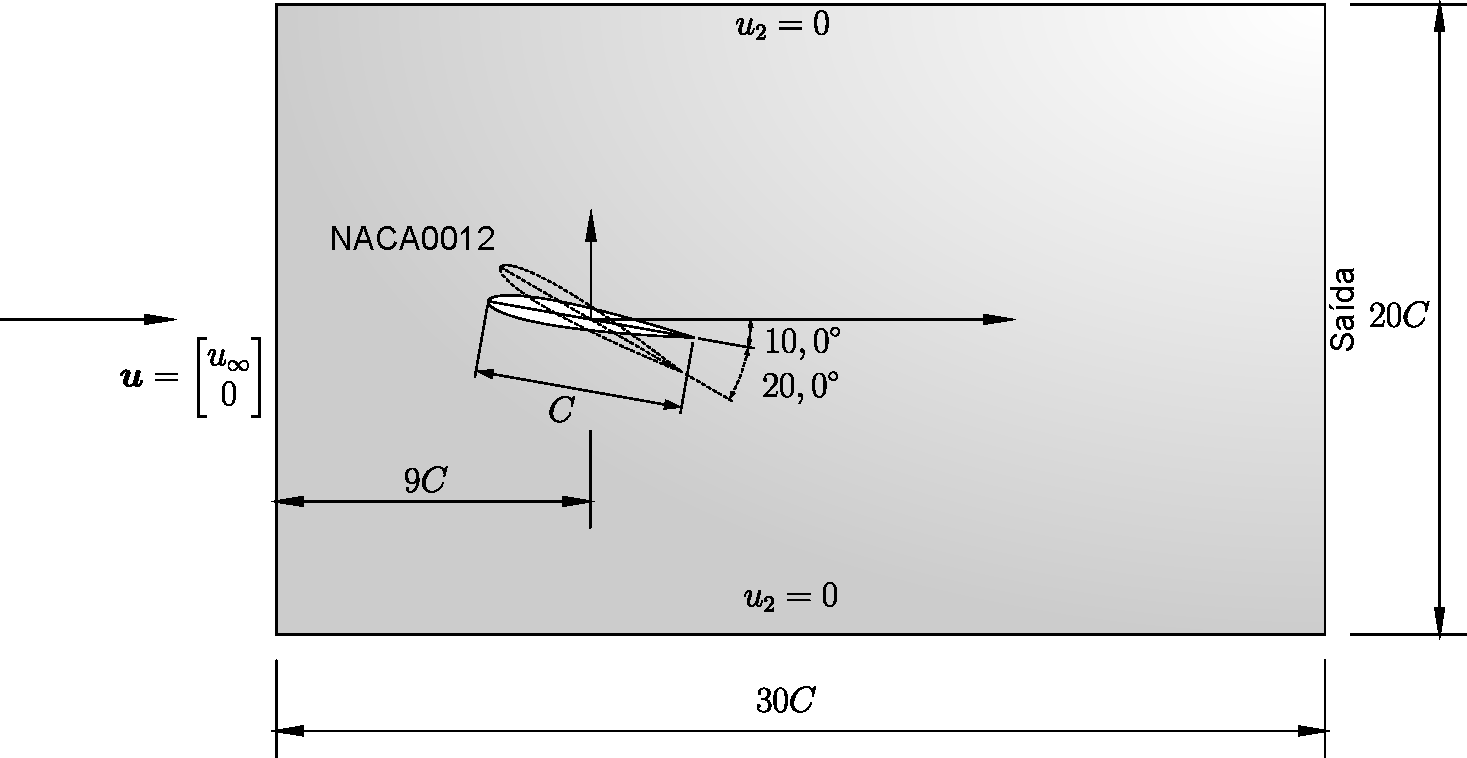
\includegraphics[width=.8\linewidth]{Figuras/rotating-airfoil/rotating-airfoil.pdf}
    \\Fonte: Autoria Própria (\the\year).
    \label{fig:rotating-airfoil}
\end{figure}

O número de Reynolds do problema, considerando o $C=1,0$ o comprimento característico do problema e baseado na velocidade de entrada $u_\infty=1,0$, é $\Rey=1000$. Para se obter a condição inicial do problema, realizou-se uma simulação estática para cada malha, mantendo-se fixo o ângulo de ataque inicial, até que se atingisse o regime permanente.

Para esse estudo, considerou-se duas malhas distintas de elementos triangulares de aproximação quadrática, a primeira (m1) contendo 3271 elementos, 6691 nós e 20073 graus de liberdade, e a segunda (m2) contendo 2743 elementos, 5597 nós e 16791 graus de liberdade. A malha m1 foi simulada em DNS (estabilizada por SUPG/PSPG), enquanto a m2 foi realizada tanto em DNS (estabilizada por SUPG/PSPG e VMS) quanto em LES (estabilizado por SUPG/PSPG). O esquema de integração temporal dado por $\rho_\infty=0,0$, o intervalo de tempo estudado é de $t\in[0,30]$ com passos de tempo $\Delta t=0,02$. A Figura \ref{fig:rotating-airfoil} apresenta as configurações iniciais da malha utilizada para ambas as simulações.

\begin{figure}[h!]
    \centering
    \caption{Aerofólio com movimento de arfagem - Configuração inicial da malha.}
    \begin{subfigure}{\linewidth}
        \centering
        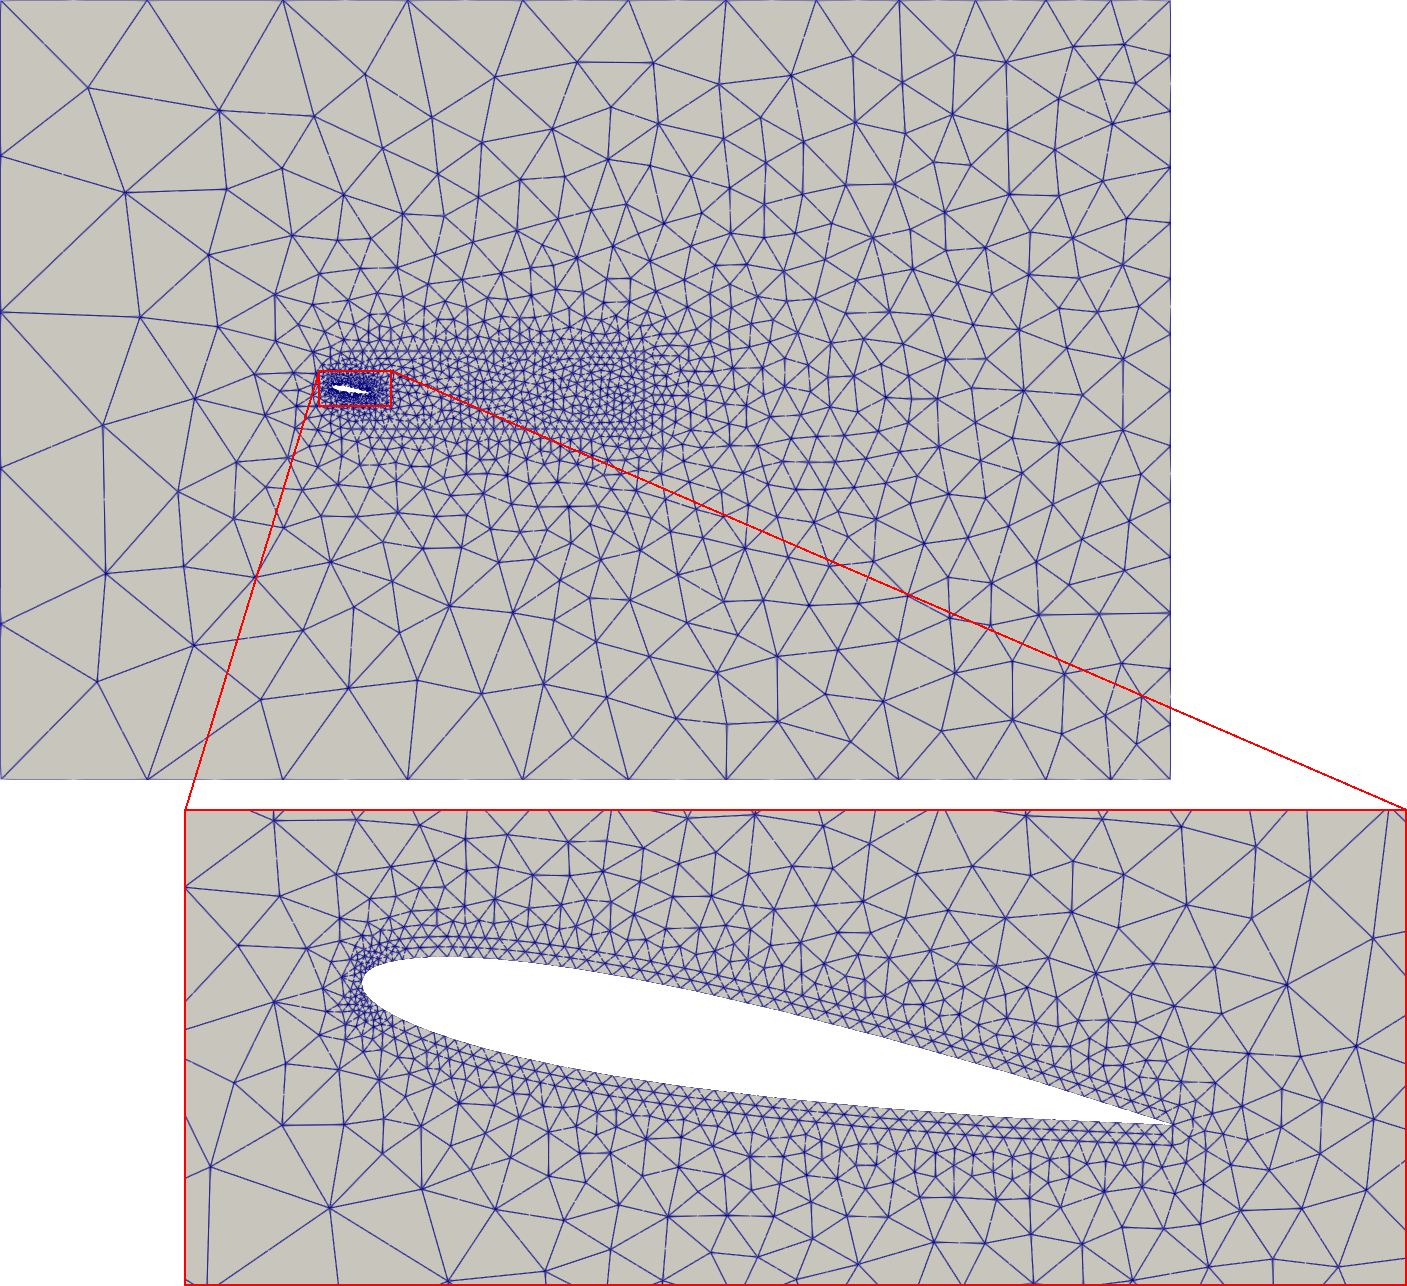
\includegraphics[width=.6\linewidth]{Figuras/rotating-airfoil/m1.png}
        \caption{Malha m1.}
    \end{subfigure}
    \begin{subfigure}{\linewidth}
        \centering
        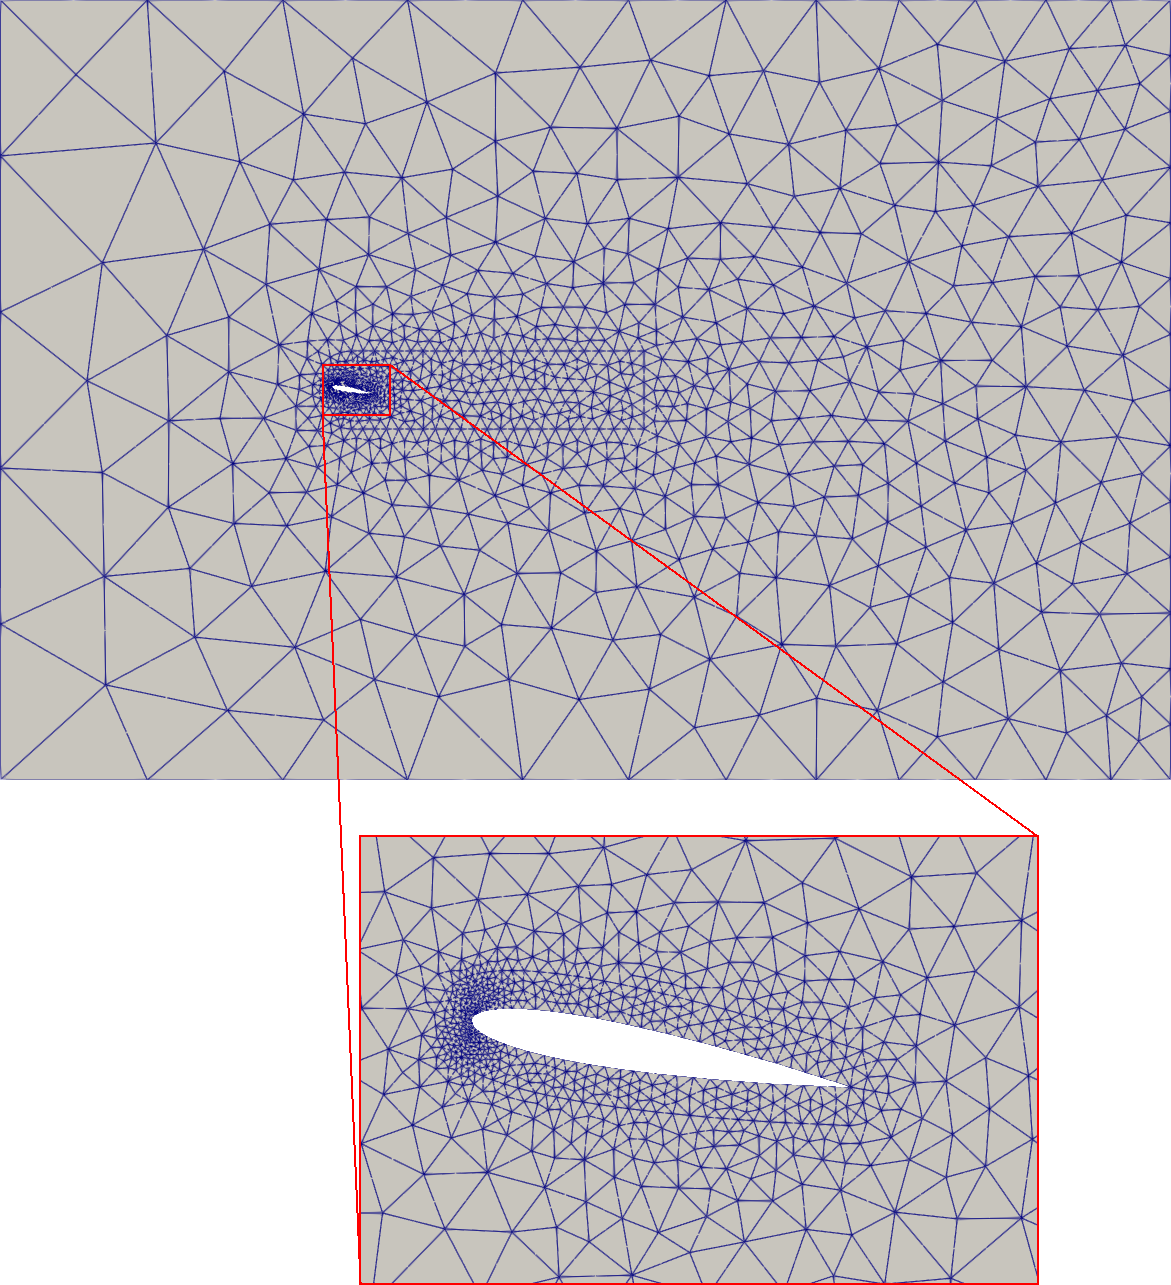
\includegraphics[width=.6\linewidth]{Figuras/rotating-airfoil/m2.png}
        \caption{Malha m2.}
    \end{subfigure}
    \\Fonte: Autoria Própria (\the\year).
    \label{fig:rotating-airfoil}
\end{figure}

Dessa maneira, observou-se os valores dos coeficientes de arrasto e de sustentação ao longo do tempo e comparou-se com os apresentados por \citeonline{mittal1992finite}. A Figura \ref{fig:rotating-airfoil-Coef} apresentam a comparação entre os resultados obtidos.

\begin{figure}[h!]
    \centering
    \caption{Aerofólio com movimento de arfagem - Evolução temporal de $C_D$ e $C_L$.}
    \begin{subfigure}{\linewidth}
        \includegraphics[width=\linewidth]{Figuras/rotating-airfoil/Cd.pdf}
        \caption{Coeficiente de arrasto.}
    \end{subfigure}
    \begin{subfigure}{\linewidth}
        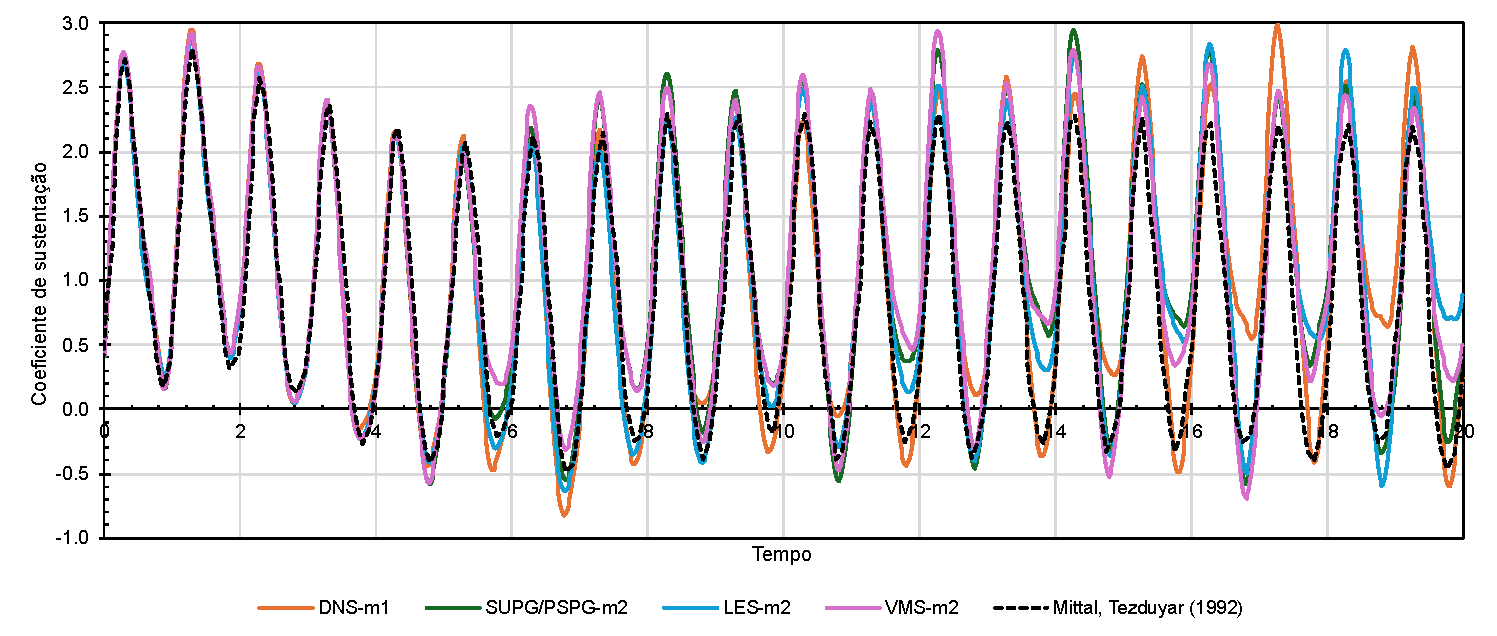
\includegraphics[width=\linewidth]{Figuras/rotating-airfoil/Cl.pdf}
        \caption{Coeficiente de sustentação.}
    \end{subfigure}
    \\Fonte: Autoria Própria (\the\year).
    \label{fig:rotating-airfoil-Coef}
\end{figure}

Pode-se observar que em todas as simulações os resultados foram muito satisfatório, se aproximando dos valores de referência. A pequena variação entre os resultados deve-se ao nível de refinamento da malha ainda ser bem adequado ao problema.

A Figura \ref{fig:vort} apresenta os campos de vorticidade e de velocidade no instante $t=8,0$ e frações de período a partir desse instante.

\begin{figure}[h!]
    \centering
    \caption{Aerofólio com movimento de arfagem - Campos de vorticidade e de velocidade.}
    \begin{subfigure}{.49\linewidth}
        \centering
        \caption*{Campo de vorticidade.}
        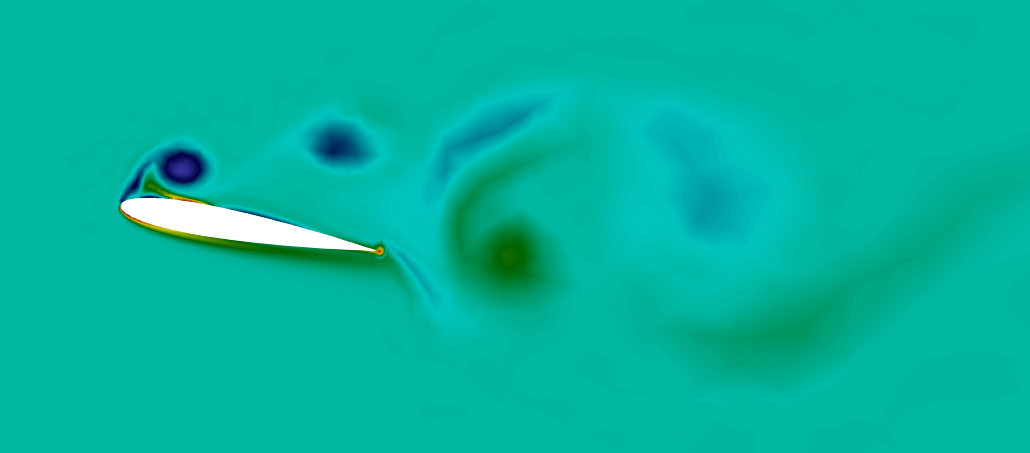
\includegraphics[width=\linewidth]{Figuras/rotating-airfoil/vort1.png}
    \end{subfigure}
    \begin{subfigure}{.49\linewidth}
        \centering
        \caption*{Campo de velocidade.}
        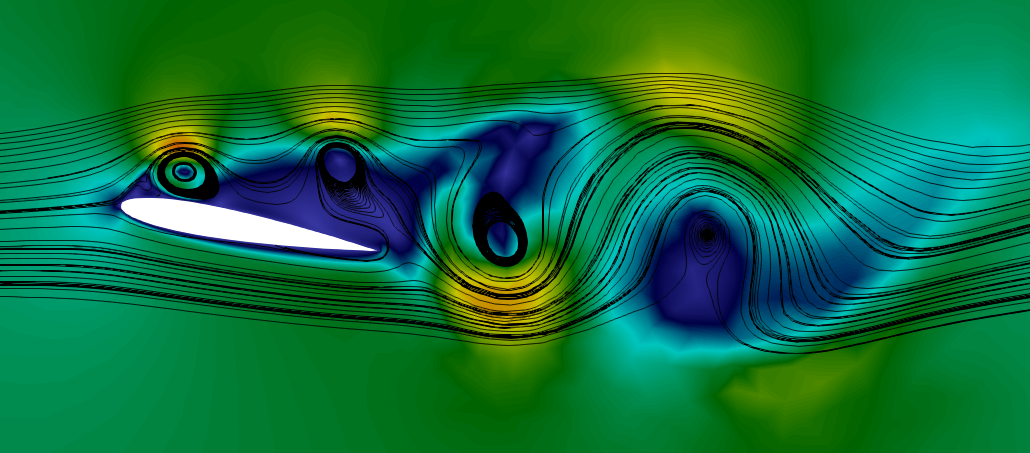
\includegraphics[width=\linewidth]{Figuras/rotating-airfoil/str1.png}
    \end{subfigure}
    \caption*{Instante $t=8,0$.}
    \begin{subfigure}{.49\linewidth}
        \centering
        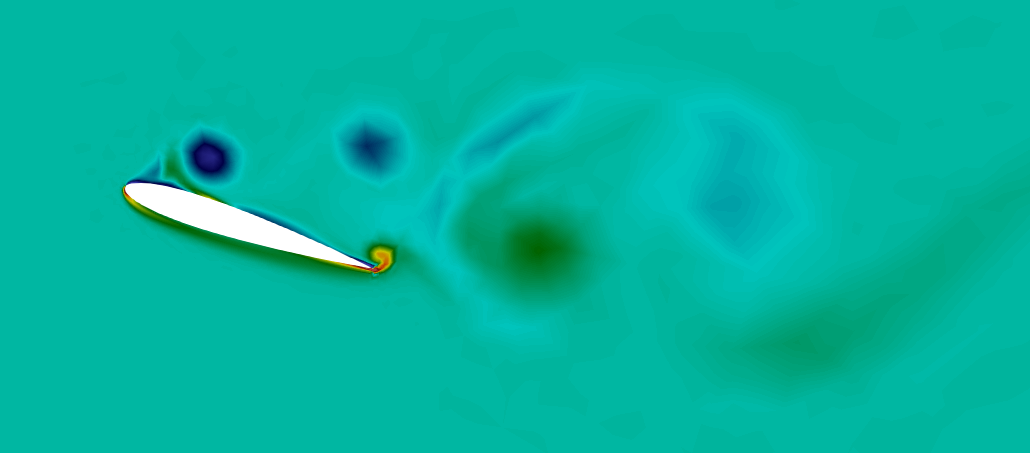
\includegraphics[width=\linewidth]{Figuras/rotating-airfoil/vort2.png}
    \end{subfigure}
    \begin{subfigure}{.49\linewidth}
        \centering
        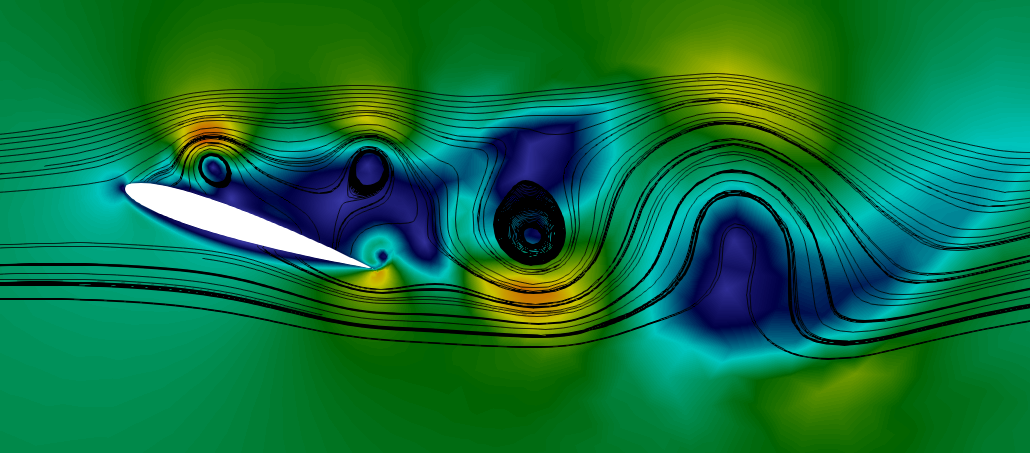
\includegraphics[width=\linewidth]{Figuras/rotating-airfoil/str2.png}
    \end{subfigure}
    \caption*{Instante $t=8,2$.}
    \begin{subfigure}{.49\linewidth}
        \centering
        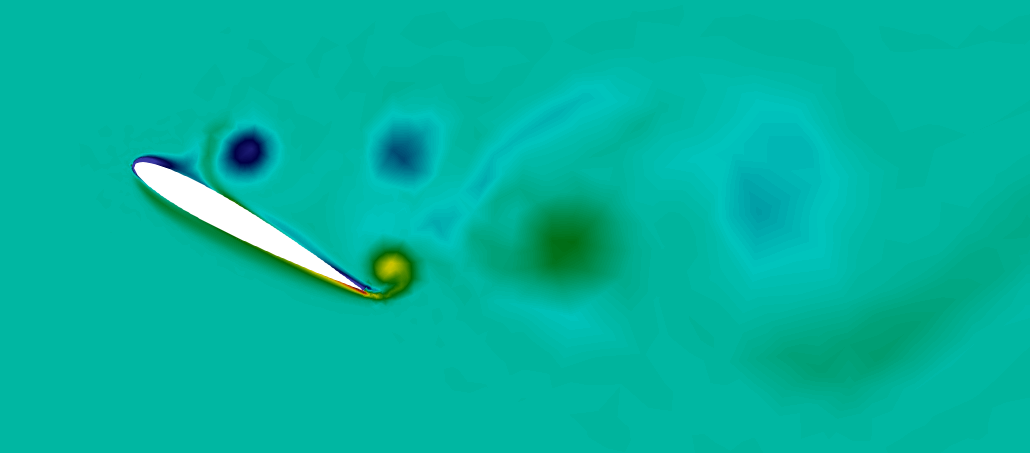
\includegraphics[width=\linewidth]{Figuras/rotating-airfoil/vort3.png}
    \end{subfigure}
    \begin{subfigure}{.49\linewidth}
        \centering
        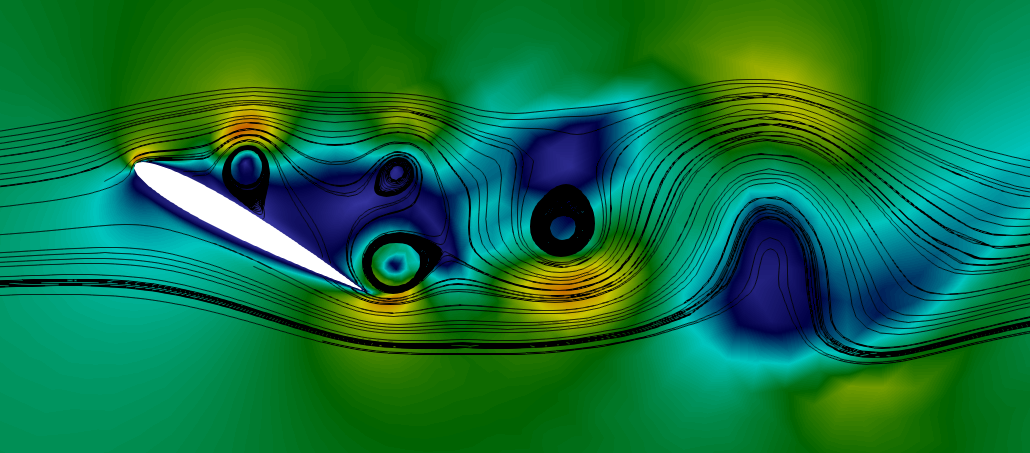
\includegraphics[width=\linewidth]{Figuras/rotating-airfoil/str3.png}
    \end{subfigure}
    \caption*{Instante $t=8,4$.}
    \begin{subfigure}{.49\linewidth}
        \centering
        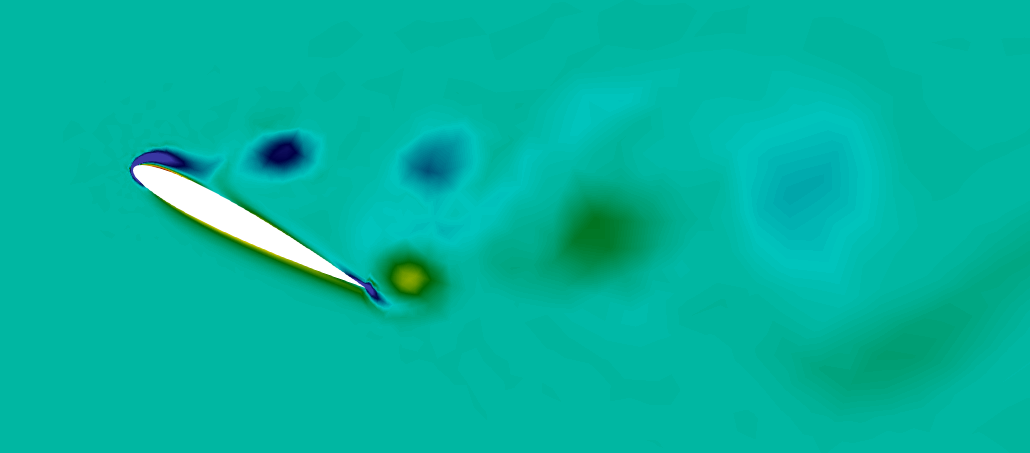
\includegraphics[width=\linewidth]{Figuras/rotating-airfoil/vort4.png}
    \end{subfigure}
    \begin{subfigure}{.49\linewidth}
        \centering
        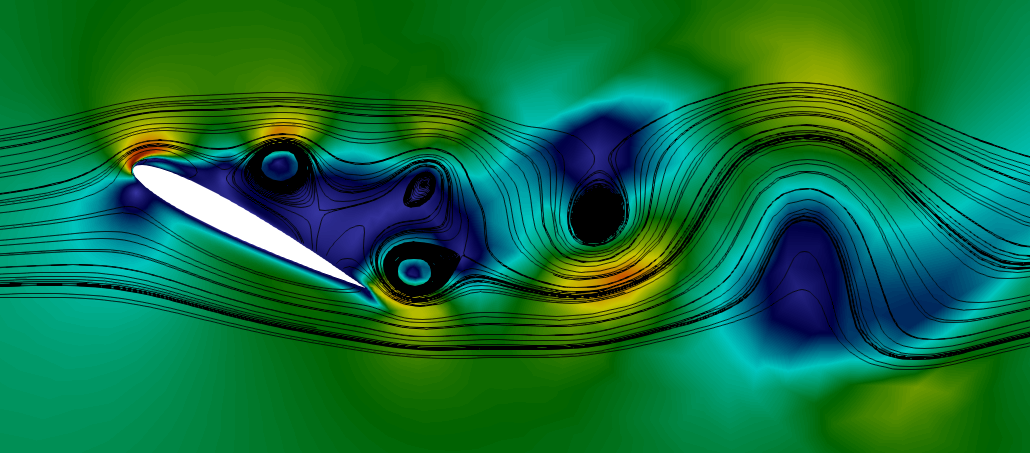
\includegraphics[width=\linewidth]{Figuras/rotating-airfoil/str4.png}
    \end{subfigure}
    \caption*{Instante $t=8,6$.}
    \begin{subfigure}{.49\linewidth}
        \centering
        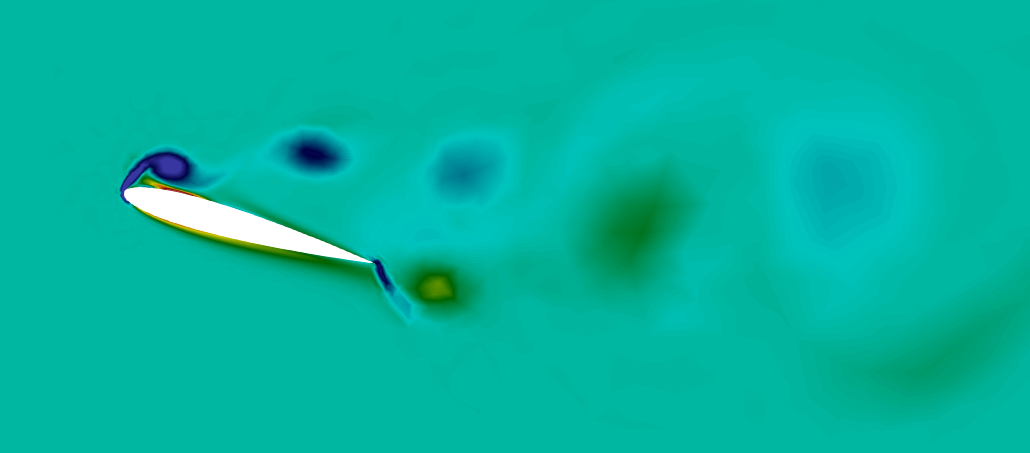
\includegraphics[width=\linewidth]{Figuras/rotating-airfoil/vort5.png}
    \end{subfigure}
    \begin{subfigure}{.49\linewidth}
        \centering
        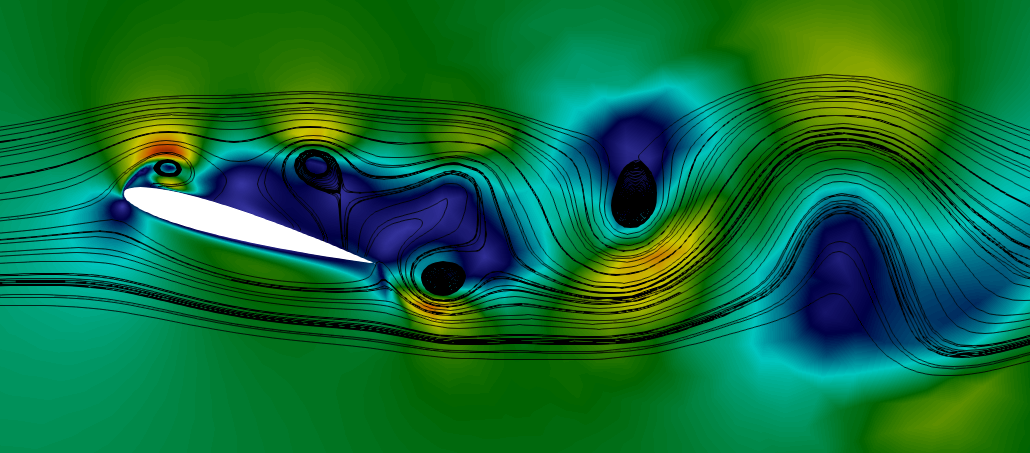
\includegraphics[width=\linewidth]{Figuras/rotating-airfoil/str5.png}
    \end{subfigure}
    \caption*{Instante $t=8,8$.}
    \begin{subfigure}{.49\linewidth}
        \centering
        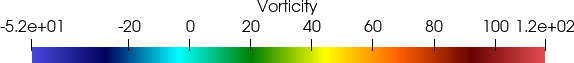
\includegraphics[width=\linewidth]{Figuras/rotating-airfoil/lvort.png}
    \end{subfigure}
    \begin{subfigure}{.49\linewidth}
        \centering
        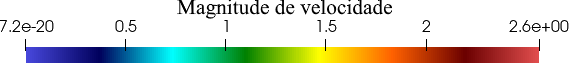
\includegraphics[width=\linewidth]{Figuras/rotating-airfoil/lstr.png}
    \end{subfigure}
    \\Fonte: Autoria Própria (\the\year).
    \label{fig:vort}
\end{figure}

Observando qualitativamente os campos são muito semelhantes aos obtidos por \citeonline{mittal1992finite}. A Figura \ref{fig:mesh} apresenta a configuração de ambas as malhas nos instantes $t=8,0$, $8,2$ e $8,4$.

\begin{figure}[h!]
    \centering
    \caption{Aerofólio com movimento de arfagem - Configuração da malha em frações de oscilação.}
    \begin{subfigure}{.49\linewidth}
        \centering
        \caption*{Malha m1.}
        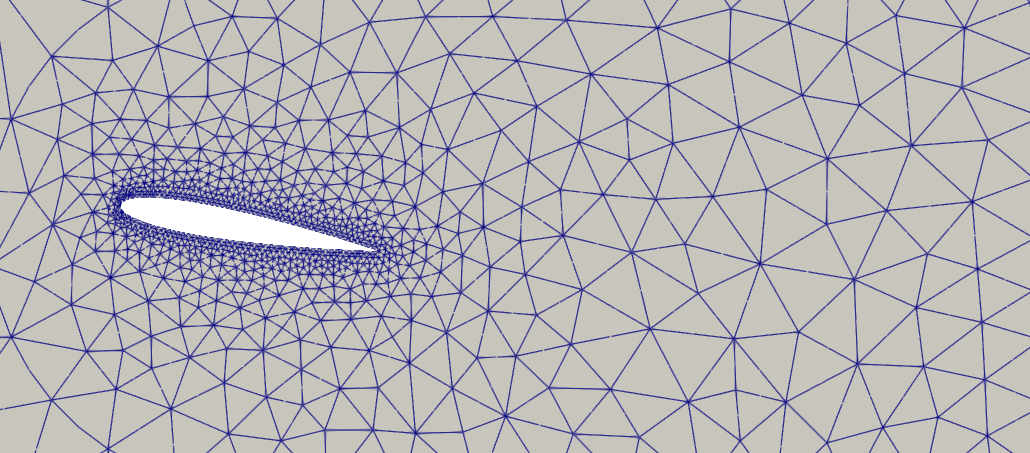
\includegraphics[width=\linewidth]{Figuras/rotating-airfoil/m11.png}
    \end{subfigure}
    \begin{subfigure}{.49\linewidth}
        \centering
        \caption*{Malha m2.}
        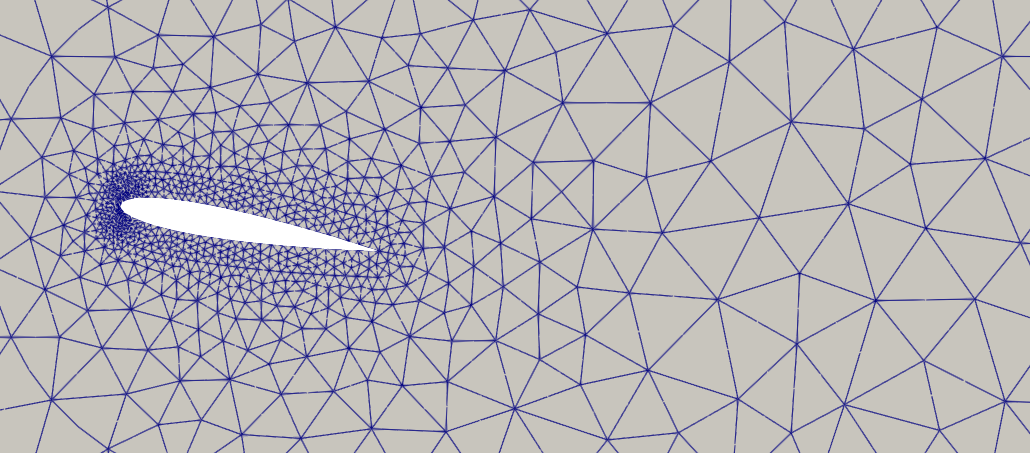
\includegraphics[width=\linewidth]{Figuras/rotating-airfoil/m21.png}
    \end{subfigure}
    \caption*{Instante $t=8,0$.}
    \begin{subfigure}{.49\linewidth}
        \centering
        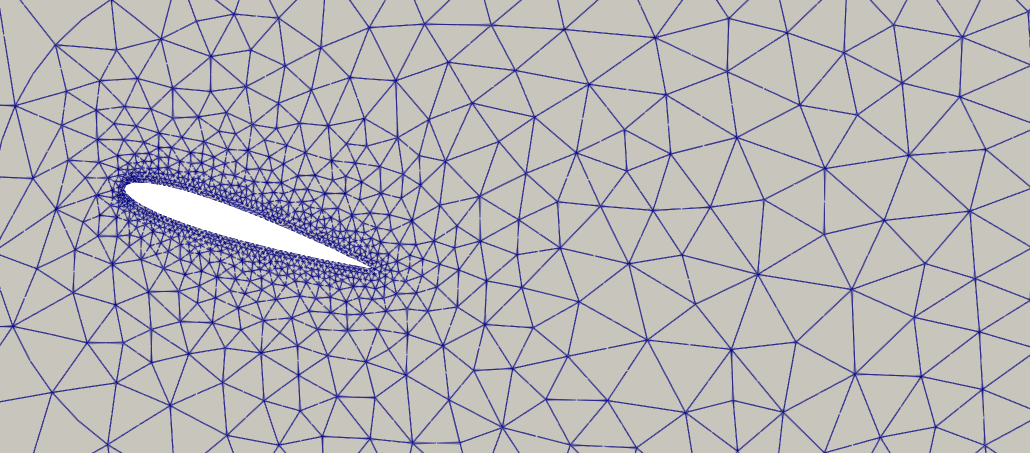
\includegraphics[width=\linewidth]{Figuras/rotating-airfoil/m12.png}
    \end{subfigure}
    \begin{subfigure}{.49\linewidth}
        \centering
        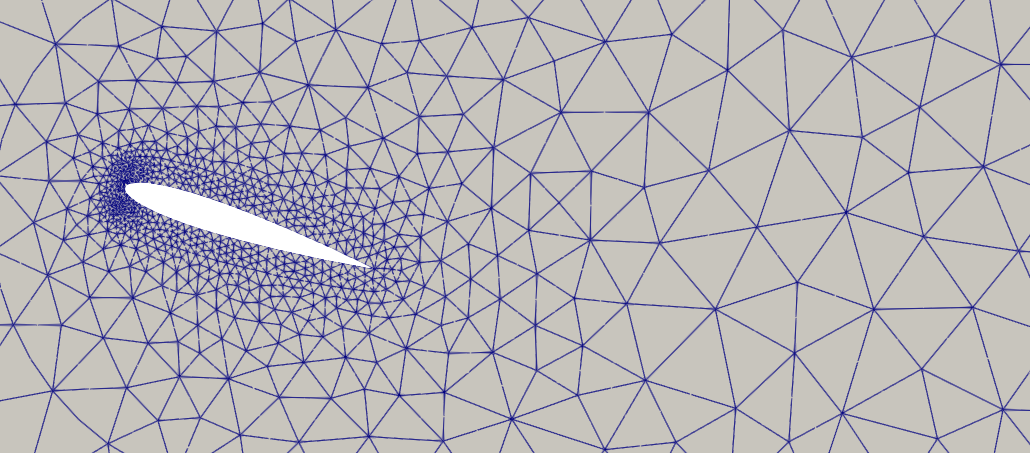
\includegraphics[width=\linewidth]{Figuras/rotating-airfoil/m22.png}
    \end{subfigure}
    \caption*{Instante $t=8,2$.}
    \begin{subfigure}{.49\linewidth}
        \centering
        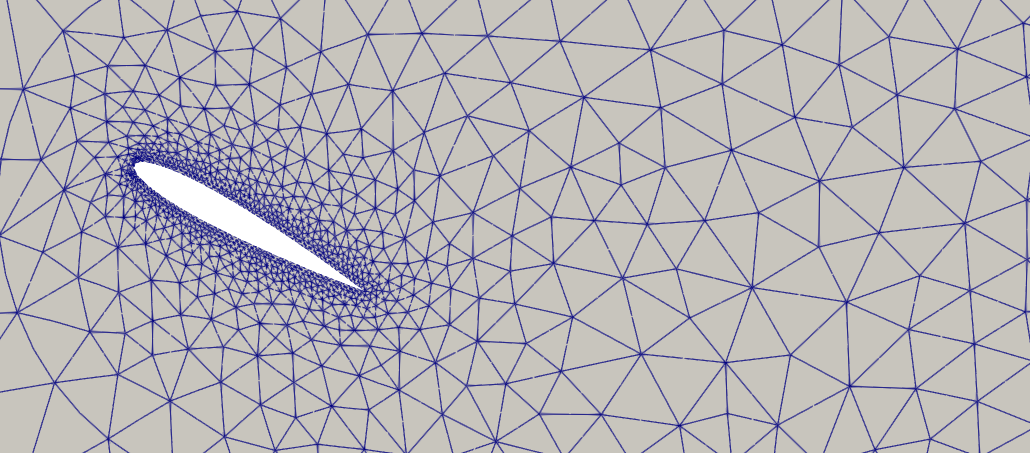
\includegraphics[width=\linewidth]{Figuras/rotating-airfoil/m13.png}
    \end{subfigure}
    \begin{subfigure}{.49\linewidth}
        \centering
        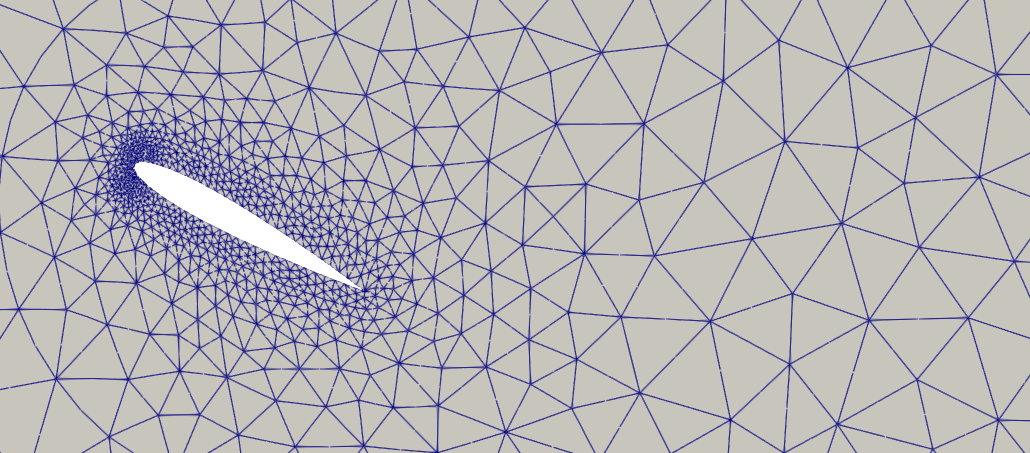
\includegraphics[width=\linewidth]{Figuras/rotating-airfoil/m23.png}
    \end{subfigure}
    \\Fonte: Autoria Própria (\the\year).
    \label{fig:mesh}
\end{figure}

Na sequência o problema foi simulado com um domínio computacional menor, o qual é esquematizado na Figura \ref{fig:rotating-airfoil-coarse}. A malha utilizada para a simulação é apresentada na Figura \ref{fig:rotating-airfoil-small-mesh}, a qual possui 1228 elementos quadráticos, 2536 nós e 7608 graus de liberdade.